%!TEX root = ../DSGEnotes.tex
\subsection{形式方程}
\label{sec:finele-form}
基于分解元$\mathcal{T}_{N}$\eqref{eq:finele-ref-decomposition},现在来分析检测空间(trial spaces)\index{trial space \dotfill 检测空间}。检测空间由分段多项式构成,这些多项式组成不同形式的基方程(base functions)\index{base function \dotfill 基方程}。基方程与全局自由度相关,不过更是在局部定义的:是针对有限元$\tau_{\ell}$,通过选取合适的形式方程(form function)\index{form function \dotfill 形式方程}而作局部定义。

考虑这样一个参考元$\tau$,它可以是一个区间($d=1$),三角形($d=2$)或是四面体($d=3$)。

\subsubsection{常数型形式方程}
最简单的形式方程可以是个常数
\begin{equation*}
  \psi_{1}^{0}(\xi) = 1, \quad \xi \in \tau,
\end{equation*}

对应地,如果有限元$\tau_{\ell}$中的某个方程$\nu_{h}(x), \, x \in \tau_{\ell}$是个常数,那么$\nu$的表现形式可写为
\begin{equation*}
  \nu_{h}(x) = \nu_{h} \left( x_{\ell_{1}} + J_{\ell} \xi \right)
  =\nu_{\ell} \, \psi_{1}^{0}(\xi), \quad x \in \tau_{\ell}, \, \xi \in \tau,
\end{equation*}
其中系数$\nu_{\ell}$反映$\nu_{h} \in \tau_{\ell}$在参考元$\tau$中对应的值。由此可得
\begin{equation}
  \label{eq:finele-form-constant-norm}
  \left\| \nu_{h} \right\|_{L^{2}(\tau_{\ell})}^{2} = \Delta_{\ell} \nu_{\ell}^{2}.
\end{equation}

\subsubsection{线性形式方程}
如果$\nu_{h}(x), \, x \in \tau_{\ell}$是个线性方程,那么$\nu_{h}$可由参考元$\tau$中结点的值$\widetilde{\nu}_{k}$所唯一决定
\begin{equation}
  \label{eq:finele-form-lin-nuh-nuk}
  \widetilde{\nu}_{h}\left( \xi \right)
  = \sum_{k=1}^{d+1} \widetilde{\nu}_{k} \psi_{k}^{1}\left( \xi \right), \quad \xi \in \tau,
\end{equation}
其中$\psi_{k}^{1}$的值如下
\begin{itemize}
  \item $d=1$时结点数$k=2$
  \begin{equation*}
    \begin{cases}
      \psi_{1}^{1} & \coloneqq 1 - \xi,\\
      \psi_{2}^{1} & \coloneqq \xi.
    \end{cases}
  \end{equation*}
  \item $d=2$时节点数$k=3$
  \begin{equation*}
    \begin{cases}
      \psi_{1}^{1} & \coloneqq 1 - \xi_{1} - \xi_{2}, \\
      \psi_{2}^{1} & \coloneqq \xi_{1}, \\
      \psi_{3}^{1} & \coloneqq \xi_{2}.
    \end{cases}
  \end{equation*}
  \item $d=3$时节点数$k=4$
  \begin{equation*}
    \begin{cases}
      \psi_{1}^{1} & \coloneqq 1 - \xi_{1} - \xi_{2} - \xi_{3}, \\
      \psi_{2}^{1} & \coloneqq \xi_{1}, \\
      \psi_{3}^{1} & \coloneqq \xi_{2}, \\
      \psi_{4}^{1} & \coloneqq \xi_{3}.
    \end{cases}
  \end{equation*}
\end{itemize}

这样一来我们有:设任意一个有限元$\tau_{\ell}$,对应结点$x_{\ell_{k}}, \, \ell_{k} \in J(\ell)$。$\tau_{\ell}$中的线性方程$\nu_{h}(x), \, x \in \tau_{\ell}$可以写为
\begin{equation}
  \label{eq:finele-form-lin-nuh-reprensentation}
  \nu_{h} \left( x \right)
  = \nu_{h} \left( x_{\ell_{1}} + J_{\ell} \xi \right)
  = \sum_{k=1}^{d+1} \nu_{\ell_{k}} \psi_{k}^{1} \left( \xi \right), \quad x \in \tau_{\ell}, \xi \in \tau.
\end{equation}

与常数形式方程的范数\eqref{eq:finele-form-constant-norm}类似,线性形式方程$\nu_{h}(x), \, x \in \tau_{\ell}$的范数$\left\| \nu_{h} \right\|_{L^{2}} \left(\tau_{\ell} \right)$也可以用结点的值$\nu_{\ell}(\xi), \, \xi \in \tau$来表示,见如下引理。
\begin{lemma}[线性形式方程的范数]
  \label{lemma:finele-form-lin-norm-def}
  设线性方程$\nu_{h}(x), \, x \in \tau_{\ell}$如\eqref{eq:finele-form-lin-nuh-reprensentation}所示。那么我们有范数不等式关系
  \begin{equation}
    \label{eq:finele-form-lin-norm-def}
    \frac{\Delta_{\ell}}{\left( d+1 \right) \left( d+2 \right)}
    \sum_{k=1}^{d+1} \nu_{\ell_{k}}^{2}
    \le \left\| \nu_{h} \right\|_{L^{2}(\tau_{\ell})}^{2}
    \le \frac{\Delta_{\ell}}{\left( d+1 \right)}
    \sum_{k=1}^{d+1} \nu_{\ell_{k}}^{2}
  \end{equation}
\end{lemma}
\begin{proof}
  线性方程$\nu_{h}(x) \in L^{2}(\tau_{\ell})$的范数
  \begin{equation*}
    \begin{split}
      \left\| \nu_{h} \right\|_{L^{2}(\tau_{\ell})}^{2}
      & = \langle \nu_{h}, \nu_{h} \rangle_{L^{2}(\tau_{\ell})} \\
      & = \sum_{i=1}^{d+1} \sum_{j=1}^{d+1} \nu_{i} \nu_{j}
      \int_{\tau} \psi_{i}\left( \xi \right) \psi_{j}\left( \xi \right) \left| \det J_{\ell} \right| \, d \xi \\
      & = \left( G_{\ell} \, \underline{\nu}^{\ell}, \underline{\nu}^{\ell} \right),
    \end{split}
  \end{equation*}
  其中$G_{\ell}$是局部质量矩阵(local mass matrix)\index{mass matrix!local \dotfill 局部质量矩阵}
  \begin{equation*}
    G_{\ell} = \frac{
    \Delta_{\ell}
    }{
    \left( d + 1 \right)\left( d + 2 \right)}
    \underbrace{
    \left(
    I_{d+1} + \underline{e}_{d+1} \underline{e}_{d+1}^{\top}
    \right)
    }_{\eqqcolon \mathcal{A}}
    , \quad \underline{e}_{d+1} = \underline{1} \in \mathbb{R}^{d+1}.
  \end{equation*}

提取$G_{\ell}$矩阵$\mathcal{A}$,计算特征值,Mathematica中代码如下
\begin{verbatim}
  d = 3 (*三维系统d=3。改为2或1,对应二维、一维系统*)
  ee = Table[1, d + 1, d + 1]
  et = Transpose[ee]
  ii = IdentityMatrix[d + 1]
  new = ii + ee*et
  Eigenvalues[new]
\end{verbatim}
可得$\lambda_{1}\left[ \mathcal{A} \right]=1, \, \lambda_{2}\left[ \mathcal{A} \right] = \ldots = \lambda_{d+1} \left[ \mathcal{A} \right] =1$。进而证得\eqref{eq:finele-form-lin-norm-def}。
\end{proof}

许多应用中需要将$\nu_{h}(x)$的斜率与$\nu_{h}(x)$自身关联起来,见下引理。
\begin{lemma}[方程范数与方程斜率的范数]
  \label{lemma:finele-form-norm-gradient}
  设线性方程$\nu_{h}$如\eqref{eq:finele-form-lin-nuh-reprensentation}所给定。则以下局部逆不等式关系成立
  \begin{equation}
    \label{eq:finele-form-norm-gradient}
    \left\| \triangledown_{x} \nu_{h} \right\|_{L^{2}(\tau_{\ell})}
    \le c_{I} h_{\ell}^{-1} \left\| \nu_{h} \right\|_{L^{2}(\tau_{\ell})},
  \end{equation}
  其中常数$c_{I} > 0$。
\end{lemma}
\begin{proof}
  分以下几步来证明。

  第一步。由Theorem \ref{theorem:finele-ref-d123-norm-equiv} 可得$\nu_{h}(x), \, x \in \tau_{\ell}$方程斜率的范,与形式方程$\widetilde{nu}_{\ell} (\xi), \, \xi \in \tau$方程斜率范的关系
\begin{equation*}
  \left\| \triangledown_{x} \nu_{h} \right\|_{L^{2}(\tau_{\ell})}^{2}
  \le c_{2} \Delta_{\ell} h_{\ell}^{-2} \,
  \left\| \triangledown_{\xi} \widetilde{\nu}_{\ell}
  \right\|_{L^{2}(\tau)}^{2}.
\end{equation*}

那么下面需要计算线性方程
\begin{equation*}
\widetilde{\nu}_{\ell} (\xi) = \sum_{k=1}^{d+1} \nu_{\ell_{k}} \psi_{k}^{1} \left( \xi \right)
\end{equation*}
的斜率以及范数。分$d=1,2,3$三种情况。
\begin{itemize}
  \item $d=1$时,
  \begin{equation*}
    \triangledown_{\xi} \widetilde{\nu}_{\ell} = \nu_{\ell_{2}} - \nu_{\ell_{1}},
  \end{equation*}
  \begin{equation*}
    \begin{split}
      \left\| \triangledown_{\xi} \widetilde{\nu} \right\|_{L^{2}(\tau_{\ell})}^{2}
      & = \left( \nu_{\ell_{2}} - \nu_{\ell_{2}} \right)^{2}
      \le 2 \left[
      \nu_{\ell_{2}}^{2} + \nu_{\ell_{1}}^{2}
      \right]
      \le 4 \left\| \nu_{h} \right\|_{L^{\infty}(\tau_{\ell})}^{2}.
    \end{split}
  \end{equation*}
  \item $d=2$时,
  \begin{equation*}
    \triangledown_{\xi} \widetilde{\nu}_{\ell} =
    \begin{pmatrix}
      \nu_{\ell_{2}} - \nu_{\ell_{1}} \\
      \nu_{\ell_{3}} - \nu_{\ell_{1}}
    \end{pmatrix},
  \end{equation*}
  \begin{equation*}
    \begin{split}
    \left\| \triangledown_{\xi} \widetilde{\nu}_{\ell} \right\|_{L^{2}(\tau)}^{2}
    & = \frac{1}{2} \,
    \left[
    \left( \nu_{\ell_{2}} - \nu_{\ell_{1}} \right)^{2} +
    \left( \nu_{\ell_{3}} - \nu_{\ell_{1}} \right)^{2}
    \right] \\
    & \le \frac{1}{2} \,
    \left[
    2 \nu_{\ell_{2}}^{2} + 2 \nu_{\ell_{3}}^{2} + 4 \nu_{\ell_{4}}^{2}
    \right] \\
    & \le 4 \, \left\| \nu_{h} \right\|_{L^{\infty}(\tau_{\ell})}.
  \end{split}
  \end{equation*}
  \item $d=3$时
  \begin{equation*}
    \triangledown_{\xi} \widetilde{\nu}_{\ell} =
    \begin{pmatrix}
      \nu_{\ell_{2}} - \nu_{\ell_{1}} \\
      \nu_{\ell_{3}} - \nu_{\ell_{1}} \\
      \nu_{\ell_{4}} - \nu_{\ell_{1}}
    \end{pmatrix},
  \end{equation*}
  \begin{equation*}
    \begin{split}
    \left\| \triangledown_{\xi} \widetilde{\nu}_{\ell} \right\|_{L^{2}(\tau)}^{2}
    & = \frac{1}{6} \,
    \left[
    \left( \nu_{\ell_{2}} - \nu_{\ell_{1}} \right)^{2} +
    \left( \nu_{\ell_{3}} - \nu_{\ell_{1}} \right)^{2} +
    \left( \nu_{\ell_{4}} - \nu_{\ell_{1}} \right)^{2}
    \right] \\
    & \le \frac{1}{6} \,
    \left[
    2 \nu_{\ell_{2}}^{2} + 2 \nu_{\ell_{3}}^{2} + 2 \nu_{\ell_{4}}^{2} + 6 \nu_{\ell_{1}}^{2}
    \right]\\
    & \le 4 \, \left\| \nu_{h} \right\|_{L^{\infty}(\tau_{\ell})}^{2}.
  \end{split}
  \end{equation*}
  \end{itemize}

汇总可得
  \begin{equation*}
    \begin{split}
      \left\| \triangledown_{x} \nu_{h} \right\|_{L^{2}(\tau_{\ell})}^{2}
      & \le c_{2} \Delta_{\ell} h_{\ell}^{-2} \,
      \left\| \triangledown_{\xi} \widetilde{\nu}_{\ell} \right\|_{L^{2}(\tau)}^{2} \\
      & \le 4 c_{2} \Delta_{\ell} h_{\ell}^{2} \left\| \nu_{h} \right\|_{L^{\infty}(\tau_{\ell})}^2,
    \end{split}
  \end{equation*}
\begin{equation*}
  \hookrightarrow \left\| \triangledown_{x} \nu_{h} \right\|_{L^{2}(\tau_{\ell})}
  \le c_{I} h_{\ell}^{-1} \,
  \left\| \nu_{h} \right\|_{L^{2}(\tau_{\ell})}.
\end{equation*}
\end{proof}

\subsubsection{二次形式方程}
更高幂次的非线性局部形式方程,可由相应的低幂次形式方程逐级地推定义而得。以二次形式方程为例,定义如下:
\begin{itemize}
  \item $d=1$时,
  \begin{equation*}
    \begin{cases}
      \psi_{1}^{2}(\xi) \coloneqq 1 - \xi, \\
      \psi_{2}^{2}(\xi) \coloneqq \xi, \\
      \psi_{3}^{2}(\xi) \coloneqq 4 \xi \left( 1 - \xi \right).
    \end{cases}
  \end{equation*}
  \item $d=2$时,
  \begin{equation*}
    \begin{cases}
      \psi_{1}^{2}(\xi) \coloneqq 1 - \xi_{1} - \xi_{2}, \\
      \psi_{2}^{2}(\xi) \coloneqq \xi_{1}, \\
      \psi_{3}^{2}(\xi) \coloneqq \xi_{2}, \\
      \psi_{4}^{2}(\xi) \coloneqq 4 \xi_{1} \left( 1 - \xi_{1} - \xi_{2} \right), \\
      \psi_{5}^{2}(\xi) \coloneqq 4 \xi_{1} \xi_{2}, \\
      \psi_{6}^{2}(\xi) \coloneqq 4 \xi_{2} \left( 1 - \xi_{1} - \xi_{2} \right).
    \end{cases}
  \end{equation*}
  \item $d=3$时,
  \begin{equation*}
    \begin{cases}
      \psi_{1}^{2}(\xi) \coloneqq 1 - \xi_{1} - \xi_{2} - \xi_{3}, \\
      \psi_{2}^{2}(\xi) \coloneqq \xi_{1}, \\
      \psi_{3}^{2}(\xi) \coloneqq \xi_{2}, \\
      \psi_{4}^{2}(\xi) \coloneqq \xi_{3}, \\
      \psi_{5}^{2}(\xi) \coloneqq 4 \xi_{1} \left( 1 - \xi_{1} - \xi_{2} - \xi_{3} \right), \\
      \psi_{6}^{2}(\xi) \coloneqq 4 \xi_{1} \xi_{2}, \\
      \psi_{7}^{2}(\xi) \coloneqq 4 \xi_{2} \left( 1 - \xi_{1} - \xi_{2} - \xi_{3} \right), \\
      \psi_{8}^{2}(\xi) \coloneqq 4 \xi_{3} \left( 1 - \xi_{1} - \xi_{2} - \xi_{3} \right), \\
      \psi_{9}^{2}(\xi) \coloneqq 4 \xi_{3} \xi_{1}, \\
      \psi_{10}^{2}(\xi) \coloneqq 4 \xi_{2} \xi_{3}.
    \end{cases}
  \end{equation*}
\end{itemize}

注意,线性形式方程与结点$x_{k} \in \overline{\tau}_{\ell}$的自由度有关,而非线性形式方程则与边的中值点$x_{k_{j}}^{*}$有关。若方程$x_{h}$在$\tau_{\ell}$中是二次形式的,那么可以写作
\begin{equation}
  \label{eq:finele-form-quadratic}
  \begin{split}
    \nu_{h}(x)
    & = \nu_{h} \left( x_{\ell_{1}} + J_{\ell} \xi \right) \\
    & = \sum_{k=1}^{\frac{1}{2} \left( d+1 \right)\left( d+2 \right)}
    \nu_{\ell_{k}} \psi_{k}^{2}(\xi), \quad \, x \in \tau_{\ell}, \, \xi \in \tau.
  \end{split}
\end{equation}

类似于Lemma \ref{lemma:finele-form-lin-norm-def},二次形式方程的范数可写作
\begin{equation*}
  \begin{split}
  \left\| \nu_{h} \right\|_{L^{2}(\tau_{\ell})}^{2}
  & = \sum_{i,j=1}^{\frac{1}{2} \left( d+1 \right) \left( d+2 \right)}
  \nu_{i} \nu_{j}
  \int_{\tau} \psi_{i}^{2}(\xi) \psi_{j}^{2}(\xi) \, \left| \det J_{\ell} \right| \, d \xi \\
  & = \left( G_{\ell} \underline{\nu}^{\ell}, \underline{\nu}^{\ell} \right),
\end{split}
\end{equation*}
\begin{itemize}
  \item $d=1$时,局部质量矩阵$G_{\ell}$为
  \begin{equation*}
    G_{\ell} =
    \begin{pmatrix}
      \frac{1}{3} & \frac{1}{6} & \frac{1}{3} \\
      \frac{1}{6} & \frac{1}{3} & \frac{1}{3} \\
      \frac{1}{3} & \frac{1}{3} & \frac{8}{15}
    \end{pmatrix},
  \end{equation*}
  对应特征值计算得
  \begin{equation*}
    \begin{split}
      \lambda_{1} &= \frac{\Delta_{\ell}}{6}, \\
      \lambda_{2} &= \Delta_{\ell} \left[ \frac{31}{60} + \frac{\sqrt{89}}{20} \right] \\
      \lambda_{2} &= \Delta_{\ell} \left[ \frac{31}{60} + \frac{\sqrt{89}}{20} \right].
    \end{split}
  \end{equation*}
  \item $d=2,3$时,
  \begin{itemize}
    \item 等价范数的估计与线性形式方程情况下的Lemma \ref{lemma:finele-form-lin-norm-def}式\eqref{eq:finele-form-lin-norm-def}一致
    \begin{equation}
      \label{eq:finele-form-quadratic-norm-def}
      c_{1} \Delta_{\ell} \sum_{k=1}^{\frac{1}{2}\left( d+1 \right)\left( d+2 \right)}
      \nu_{\ell_{k}}^{2}
      \le \left\| \nu_{h} \right\|_{L^{2}(\tau_{\ell})}^{2}
      \le c_{2} \Delta_{\ell} \sum_{k=1}^{\frac{1}{2}\left( d+1 \right)\left( d+2 \right)}
      \nu_{\ell_{k}}^{2},
    \end{equation}
    其中二次形式方程$\nu_{h}$的定义如\eqref{eq:finele-form-quadratic}。
    \item 逆不等式也与线性形式下的情况Lemma \ref{lemma:finele-form-norm-gradient}式\eqref{eq:finele-form-norm-gradient}相一致。
  \end{itemize}
\end{itemize}


\subsection{检测空间}
\label{sec:finele-trial}
对于二阶偏微分方程的边界值问题,为了计算近似解,需要我们构建检测空间$\mathcal{S}_{h}^{1}\left(\mathcal{T}_{N} \right)$,空间中包括局部分段线性方程和全局连续方程。

对于容许分解\eqref{eq:finele-ref-decomposition}来说,在分解产生的结点$x_{k}$处,$\mathcal{S}_{h}^{1}\left(\mathcal{T}_{N} \right)$便由结块方程(nodal function)所唯一确定,$\nu_{k} = \nu_{h}(x_{k})$。通过这样的方式,可以将有限元$\tau_{\ell}$用局部形式方程予以表现。

全局检测空间$\mathcal{S}_{h}^{1}\left(\mathcal{T}_{N} \right)$的维数$\dimm \mathcal{S}_{h}^{1}\left(\mathcal{T}_{N} \right)$也因此等于分解后的结点数。对应地,$\mathcal{S}_{h}^{1}\left(\mathcal{T}_{N} \right)$的基$\psi_{k}^{1}(x)$如图所示,可以写为
\begin{equation*}
  \psi_{k}^{1} (x) \coloneqq
  \begin{cases}
  1 & x = x_{k}, \\
  0 & x = x_{\ell} \neq x_{k}, \\
  \text{线性} & \text{其他情况}.
\end{cases}
\end{equation*}

\begin{figure}[htbp]
  \centering
  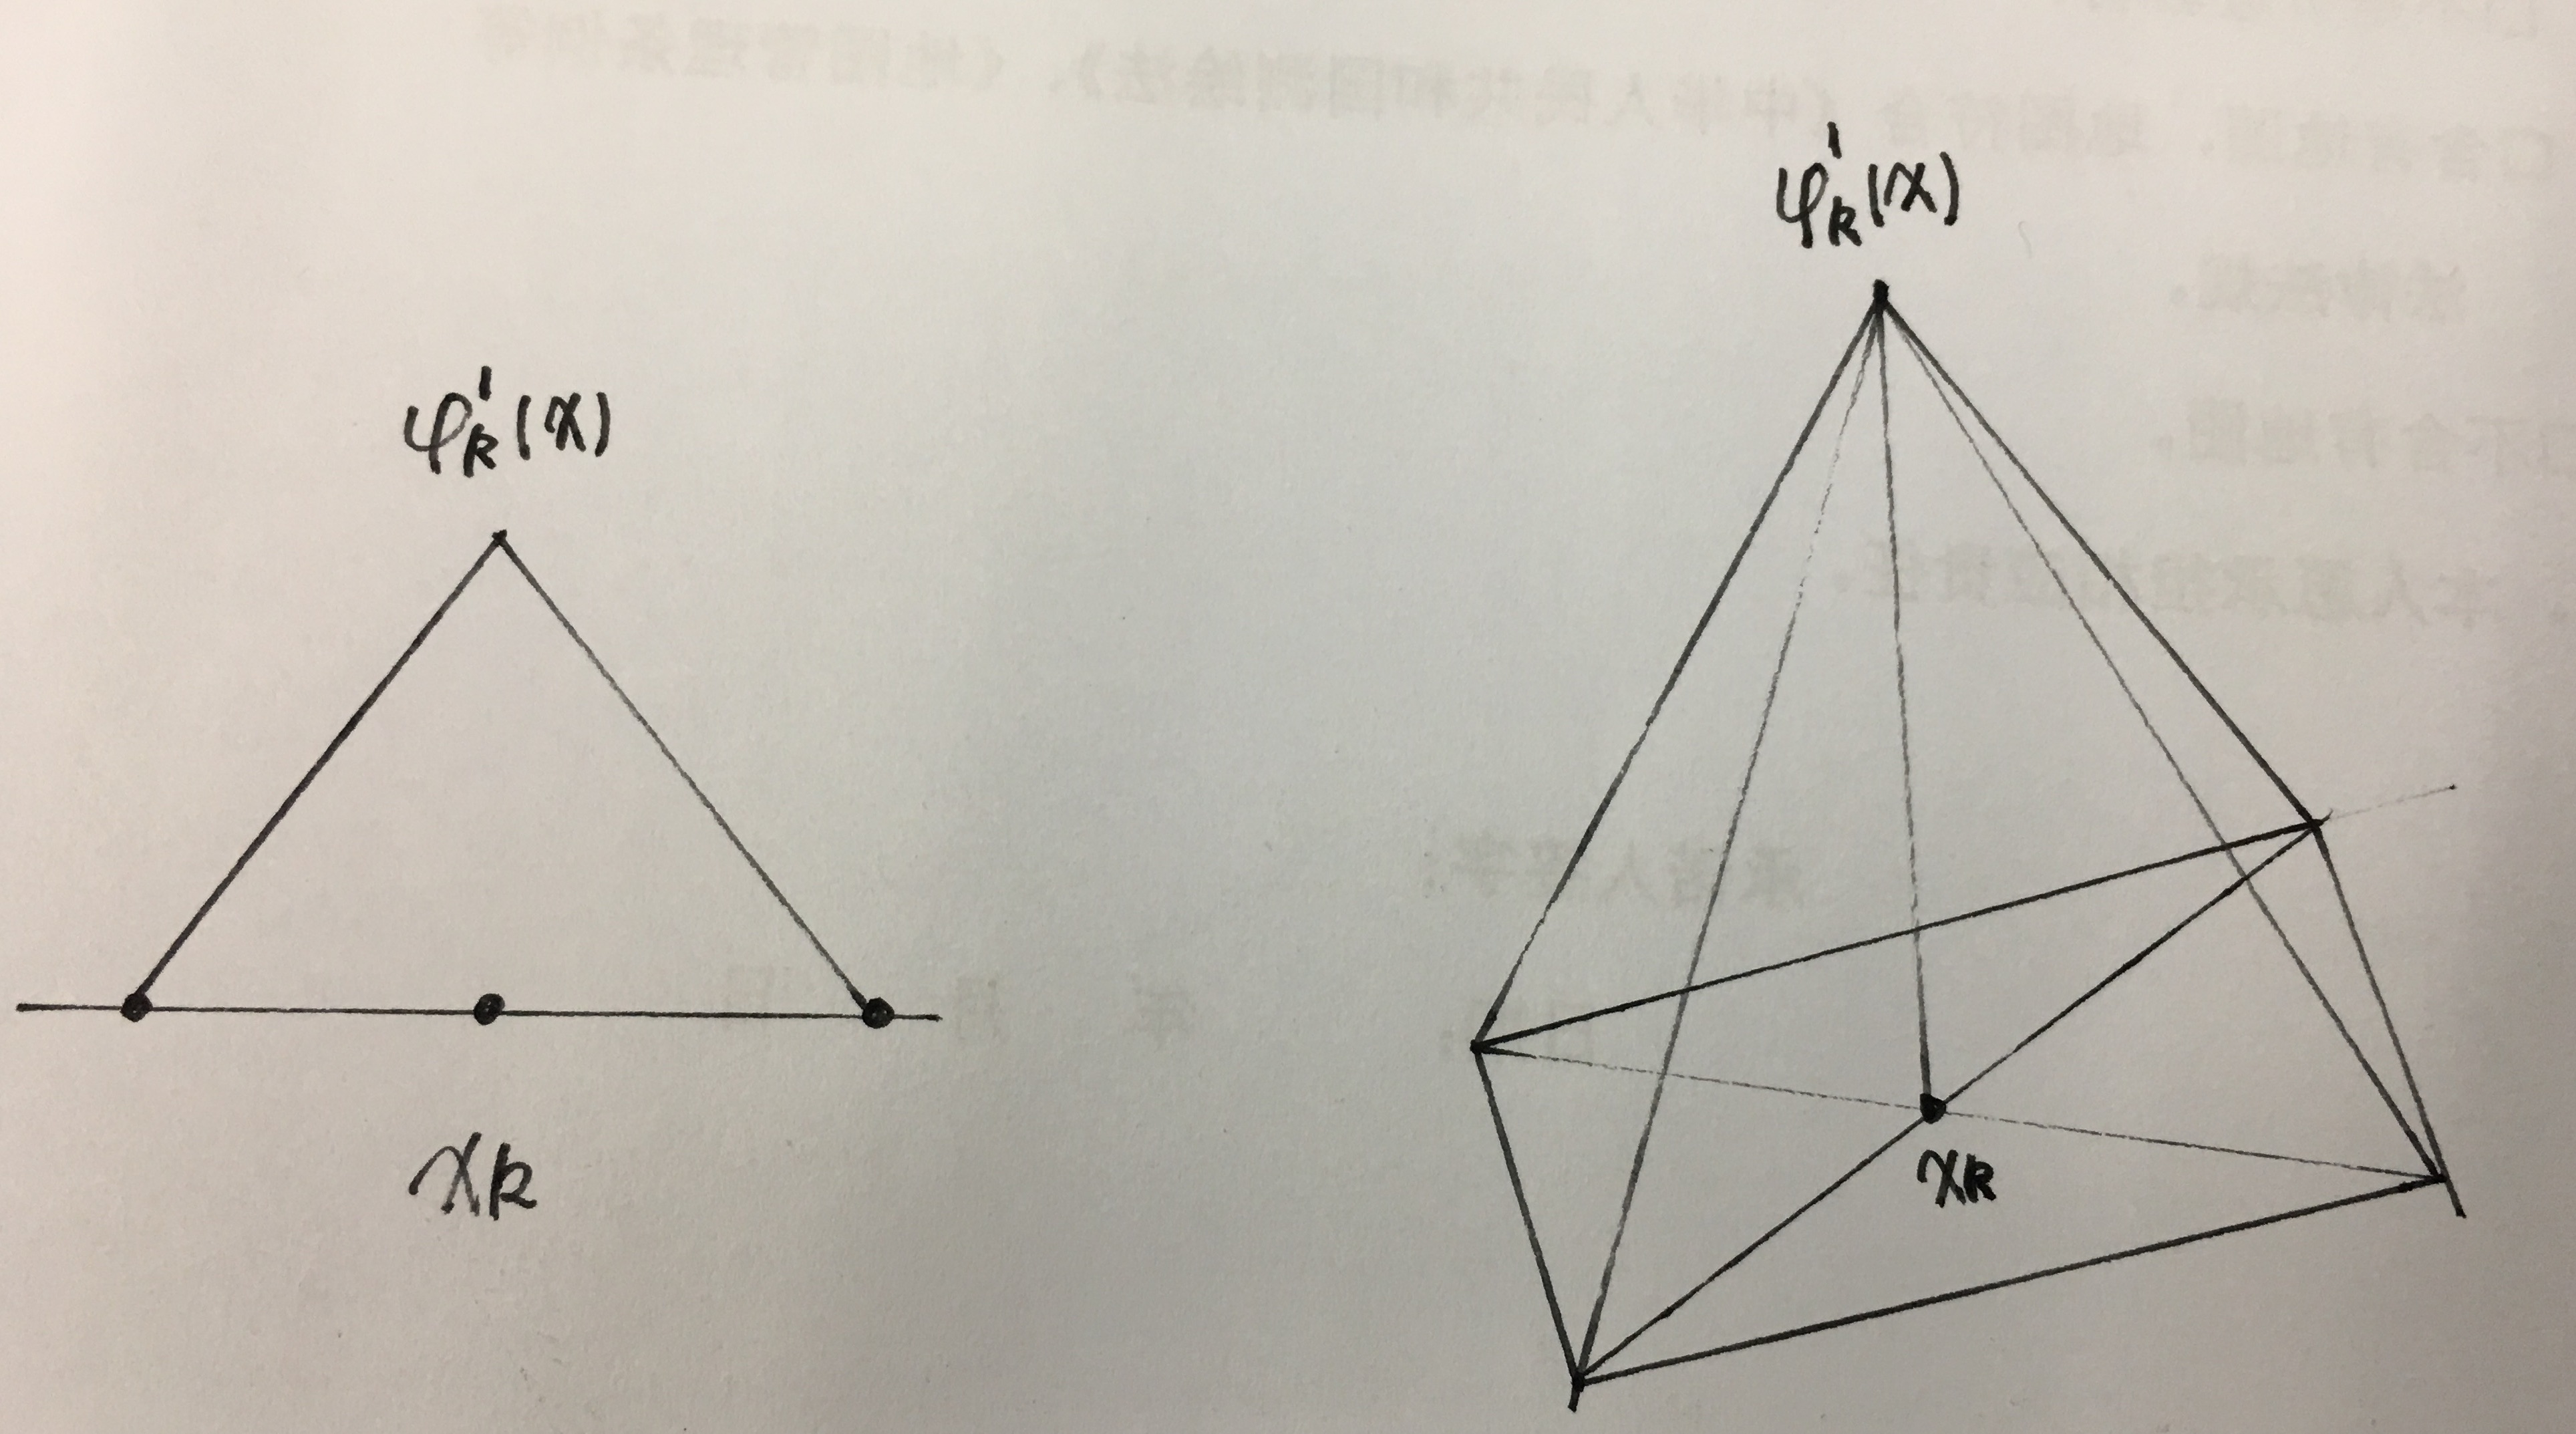
\includegraphics[width=4in]{./figures/20171214-trial-space-basis}
 \caption{检测空间$\mathcal{S}_{h}^{1}\left(\mathcal{T}_{N} \right)$的基$\psi_{k}^{1}(x)$}
\label{fig:finele-trial-basis}

%  \small{注:实线表示名义资金流动。虚线表示实际物质流动。}
\end{figure}


分段线性方程$\nu_{h}(x) \in \mathcal{S}_{h}^{1}\left(\mathcal{T}_{N} \right)$可以表示为
\begin{equation*}
  \nu_{h}(x) = \sum_{k=1}^{M} \nu_{k} \psi_{k}^{1}(x).
\end{equation*}

进而检测空间中的范数见下引理
\begin{lemma}[光谱等价范数不等式]
  \label{lemma:finele-trial-norm-spectral}
  $\nu_{h}(x) \in \mathcal{S}_{h}^{1}\left(\mathcal{T}_{N} \right)$在分解中的光谱等价范数不等式为
  \begin{equation}
    \label{eq:finele-trial-norm-spectral}
    \begin{split}
      \frac{1}{\left( d+1 \right)\left( d+2 \right)}
      \sum_{k=1}^{M}
      \left(\sum_{\ell \in I(k)} \Delta_{\ell} \right)
      \nu_{k}^{2}
      \le \left\|\nu_{h}\right\|_{L^{2}\left(\mathcal{T}_{N} \right)}
      \le \frac{1}{\left( d+1 \right)}
      \sum_{k=1}^{M}
      \left(\sum_{\ell \in I(k)} \Delta_{\ell} \right)
      \nu_{k}^{2}.
    \end{split}
  \end{equation}
\end{lemma}
\begin{proof}
  由Lemma \ref{lemma:finele-form-lin-norm-def}可得
  \begin{equation*}
    \begin{split}
      \left\| \nu_{h} \right\|_{L^{2} \left( \mathcal{T}_{N} \right)}^{2}
      & = \sum_{\ell}^{N} \left\| \nu_{h} \right\}
      \left\| \nu_{h} \right\|_{L^{2} \left( \mathcal{T}_{\ell} \right)}^{2} \\
      & \le \sum_{\ell=1}^{N}
      \frac{\Delta_{\ell}}{d+1} \,
      \sum_{k=1}^{d+1} \nu_{\ell_{k}}^{2} \\
      & = \frac{1}{d+1} \,
      \sum_{k=1}^{M} \left( \sum_{\ell \in I(k)}  \Delta_{\ell} \right)
      \nu_{k}^{2}
    \end{split}
  \end{equation*}
  为上限界。采用类似的方法可得下限界。证得\eqref{eq:finele-trial-norm-spectral}。
\end{proof}

\begin{lemma}[逆等价范数不等式]
  \label{finele-trial-norm-inverse}
  $\nu_{h}(x) \in \mathcal{S}_{h}^{1}\left(\mathcal{T}_{N} \right)$在分解中的逆等价范数不等式为
  \begin{equation}
    \label{eq:finele-trial-norm-inverse-local}
    \left\| \triangledown_{x} \nu_{h} \right\|_{L^{2} \left(\mathcal{T}_{N} \right)}^{2}
    \le c_{I} \sum_{\ell=1}^{N} h_{\ell}^{-2} \,
    \left\| \nu_{h} \right\|_{L^{2}(\tau_{\ell} )}^{2}.
  \end{equation}

  如果分解是全局拟一致的\index{quansi-uniform!globally \dotfill 全局拟一致},见\eqref{eq:finele-ref-quasi-uniform},那么我们有
  \begin{equation}
    \label{eq:finele-trial-norm-inverse-global}
    \left\| \triangledown_{x} \nu_{h} \right\|_{L^{2} \left(\mathcal{T}_{N} \right)}
    \le c \, h^{-1} \,
    \left\| \nu_{h} \right\|_{\left( \mathcal{T}_{N} \right)}.
  \end{equation}
\end{lemma}
\begin{proof}
可由Lemma  \ref{lemma:finele-form-norm-gradient}直接求得。
\end{proof}

为了求得检测空间$\mathcal{S}_{h}^{1}\left(\mathcal{T}_{N} \right)$的近似特性,首先要定义相应的插值算子和投影算子,然后计算误差测度项。
\subsubsection{检测空间的插值算子}
\label{sec:finele-trial-interpolation}
设$\nu \in C \left( \mathcal{T}_{N} \right)$是一个全局连续的方程。在含有分段线性方程的空间中定义插值如下
\begin{equation}
  \label{eq:finele-trial-interpolation}
  I_{h} \nu(x) \coloneqq \sum_{k=1}^{M} \nu(x_{k}) \varphi_{k}(x) \in  \mathcal{S}_{h}^{1}\left(\mathcal{T}_{N} \right).
\end{equation}

\begin{lemma}[分段线性插值的局部误差测度项]
  \label{lemma:finele-trial-interpolation-error}
  设给定的$\nu_{|_{\tau_{\ell}}} \in H^{2}\left( \tau_{\ell} \right)$。则我们有局部误差测度项
  \begin{equation}
    \label{eq:finele-trial-interpolation-error}
    \left\| \nu - I_{h} \nu \right\|_{L^{2}(\tau_{\ell})}
    \le c \, h_{\ell}^{2} \, \left| \nu \right|_{h^{2}(\tau_{\ell})}.
  \end{equation}
\end{lemma}
\begin{proof}
  \begin{enumerate}
  \item 根据识别方程等价范的测度不等式Theorem \ref{theorem:finele-ref-d123-norm-equiv}可得
  \begin{equation*}
  \left\| \nu - I_{h} \nu \right\|_{L^{2}(\tau_{\ell})}
  \le c \, \Delta_{\ell} \,
  \left\| \widetilde{\nu}_{\ell} - I_{\tau} \widetilde{\nu}_{\ell} \right\|_{L^{2}(\tau)},
  \end{equation*}
  其中$I_{\tau}:H^{2}(\tau) \mapsto L^{2}(\tau)$是相应参考元$\tau$的线性插值算子,满足
  \begin{equation*}
    \left\| I_{\tau} \widetilde{\nu}_{\ell} \right\|_{L^{2}(\tau)}
    \le \meas(\tau) \, \left\| \widetilde{\nu}_{\ell} \right\|_{L^{\infty}(\tau)},
  \end{equation*}
  $\meas(\tau)$表示$\tau$的测度(measure)。
  由索伯列夫嵌入定理(第\pageref{sec:imbedding-sobolev}页\ref{sec:imbedding-sobolev}节)可得
  \begin{equation*}
    \left\| \widetilde{\nu}_{\ell} \right\|_{L^{\infty}(\tau)}
    \le c \, \left\| \widetilde{\nu}_{\ell} \right\|_{L^{2}(\tau)},
  \end{equation*}
  可见$I_{\tau}:H^{2}(\tau) \mapsto L^{2}(\tau)$有界。

  \item 对于任意且固定的方程$\omega \in L^{2}(\tau)$,可定义一个线性泛函如下
  \begin{equation*}
    f(u) \coloneqq \int_{\tau} \left[
    \left( I - I_{\tau} \right) u(\xi)
    \right] \omega(\xi) d \xi.
  \end{equation*}

  如果给定方程$u \in H^{2}(\tau)$,那么我们有
  \begin{equation*}
    \begin{split}
      \left| f(u) \right|
      & = \left|
      \int_{\tau} \left[
      \left( I - I_{\tau} \right) u(\xi)
      \right]
      \omega(\xi) \, d \xi
      \right| \\
      & \le \left\|
      \left( I - I_{\tau} \right) u
      \right\|_{L^{2}(\tau)} \,
      \left\| \omega \right\|_{L^{2}(\tau)} \\
      & \le c \, \left\| u \right\|_{H^{2}(\tau)} \, \left\| \omega \right\|_{L^{2}(\tau)},
    \end{split}
  \end{equation*}
  即线性泛函$f$有界。

  对于任一线性方程$q \in \mathcal{P}_{1}(\tau)$,我们有$I_{\tau} q = q$,因此
  \begin{equation*}
    f(q) = 0, \quad \forall \, q \in \mathcal{P}_{1}(\tau).
  \end{equation*}

  可见Bramble-Hilbert引理 Lemma \ref{lemma:bramble-hilbert-lemma}的全部前提条件均得到满足。根据该引理可得
  \begin{equation*}
    \left| f(u) \right| \le \widetilde{c} \, \left\| \omega \right\|_{L^{2}(\tau)} \, \left| u \right|_{H^{2}(\tau)}.
  \end{equation*}

  \item 定义$u(\xi)$和$\omega(\xi)$的值如下
  \begin{equation*}
    \begin{cases}
      u \coloneqq \widetilde{\nu}_{\ell}, \\
      \omega \coloneqq \left( I - I_{\ell} \right) \widetilde{\nu}_{\ell},
    \end{cases}
  \end{equation*}

  进而
  \begin{equation*}
    \begin{split}
      \left\| \omega \right\|_{L^{2}(\tau)}^{2}
      & = \int_{\tau} \left( \omega (\xi) \right)^{2} d \xi
      = \int_{\tau} \left[
      \left( I - I_{\tau} \right)
      \widetilde{\nu}_{\ell}(\xi)
      \right] \omega(\xi) \, d \xi
      = \int_{\tau} \left[
      \left( I - I_{\tau} \right) u(\xi)
      \right]
      \omega(\xi) \, d \xi
      = \left| f \left( \widetilde{\nu}_{\ell} \right) \right| \\
      & \le \widetilde{c} \,
      \left\| \omega \right\|_{L^{2}(\tau)}
      \left| \widetilde{\nu}_{\ell} \right|_{H^{2}(\tau)} = \widetilde{c} \,
%      \underbrace{
      \left\| \left( I - I_{\tau} \right) \widetilde{\nu}_{\ell} \right\|_{L^{2}(\tau)}
%      }_{\eqqcolon \mathcal{A}} \,
      \, \left| \widetilde{\nu}_{\ell} \right|_{H^{2}(\tau)},
    \end{split}
  \end{equation*}
  \begin{equation*}
    \hookrightarrow
    \left\| \left( I - I_{\tau} \right) \widetilde{\nu}_{\ell} \right\|_{L^{2}(\tau)} \le \widetilde{c} \, \left| \widetilde{\nu}_{\ell} \right|_{H^{2}(\tau)}.
  \end{equation*}
  \item 代入Theorem \ref{theorem:finele-ref-d123-norm-equiv}可得
  \begin{equation*}
    \begin{split}
      \left\| \nu - I_{h} \nu \right\|_{L^{2}(\tau)}
      & \le c \, \Delta_{\ell} \,
      \left\| \widetilde{\nu}_{\ell} \right\|_{H^{2}(\tau)} \\
      & \le \hat{c} \, h_{\ell}^{2} \, \left| \nu \right|_{H^{2}(\tau_{\ell})}.
    \end{split}
  \end{equation*}
\end{enumerate}
\end{proof}

由Lemma \ref{lemma:finele-trial-interpolation-error}可得分段线性插值的全局误差项
\begin{equation}
  \label{eq:finele-trial-interpolation-error-global-L}
  \left\|
  \nu - I_{h} \nu
  \right\|_{L^{2}(\mathcal{T}_{N})}^{2}
  \le c \, \sum_{\ell=1}^{\ell} h_{\ell}^{4} \, \left| \nu \right|_{H^{2}(\tau_{\ell})}^{2},
\end{equation}
以及
\begin{equation}
  \label{eq:finele-trial-interpolation-error-global-H}
  \left\|
  \nu - I_{h} \nu
  \right\|_{H^{1}(\mathcal{T}_{N})}^{2}
  \le c \, \sum_{\ell=1}^{\ell} h_{\ell}^{2} \, \left| \nu \right|_{H^{2}(\tau_{\ell})}^{2}.
\end{equation}

\subsubsection{检测空间的投影算子}
\label{sec:finele-trial-projection}
为了应用插值算子执行上述运算,需要假定待差值的方程$\nu \in C \left( \mathcal{T}_{N} \right)$是全局连续的,这个假设过于强硬,有时较难满足。一个替代方案是以下若假设:
